\chapter{Implementation \& Evaluation}
\label{ch:impl_eval}

\begin{comment}
\section{Baseline with MCTS}
In order to develop a non-trivial strategy for an enemy playing the game(s) developed in chapter \ref{ch:modelling}, we'll use  the MCTS algorithm described in section \ref{sec:intro_mcts}.
While we could use MCTS in stead of MARL algorithms, MCTS does have some properties that make it unsuitable for our purposes. Firstly, it uses the complete state information of the game. Secondly, while it generally outperforms simpler algorithms like minimax, it still doesn't scale to more realistic situations. Furthermore, since MCTS works on turn-based games, the game from chapter \ref{ch:modelling} is adapted to accommodate executing actions in sequence for the two players.\\

However, it does allow us to develop strategies for two opposing players form the ground up. Thus using MCTS at this phase has two purposes:
\begin{enumerate}
    \item Analyzing the performance of the algorithm
    \item Obtaining a baseline opponent policy against which the MARL algorithms can be evaluated.
\end{enumerate}

\end{comment}
% ----------------------------------------------------------------------------------------

%\section{Innateness vs. Learned}
%\textbf{Discuss advantages / disadvantages of innate knowledge (e.g. no aim/fire when not in range $\rightarrow$ might be valid initial knowledge, while simple strategies might not)} 

\section{Notes on implementation}
This section describes a couple of technical points about the implementation of the algorithms of chapter \ref{ch:algorithms}.
\begin{itemize}
    \item Because of the structure of the observation that the environment provides to an agent (see \ref{sec:first_model}), all (learning) agents can use the same network to compute their policy or to estimate Q-values. This is known as \emph{weight sharing} and improves the sample efficiency since only one common network must be trained instead of a network per agent.
    \item This common network takes as input a tensor constructed from the observation and puts it through a fully-connected layer. The output for this layer is than fed to a GRU. At every time step, the hidden state of the GRU is transformed via another fully-connected layer into the policy and/or the estimated $V$- or $Q$-values, depending on the type of algorithm. The entire network for an actor-critic agent, which does both value estimation as policy prediction, is schematically represented in figure \ref{fig:agent_net}. 
    \begin{figure}[htp]
        \centering
        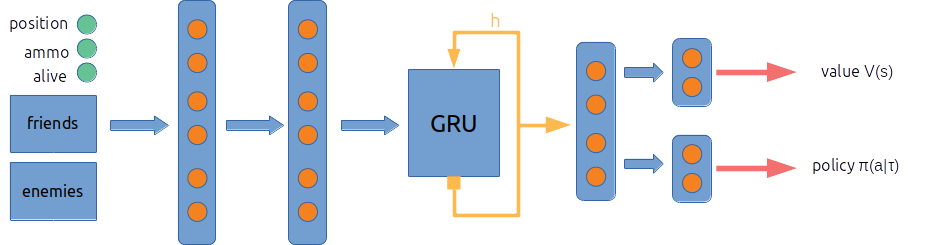
\includegraphics[width=14cm]{images/agent_net2.png}
        \caption{Actor-critic agent with a recurrent net}
        \label{fig:agent_net}
    \end{figure}
    \\A REINFORCE network only has the policy output. A Q-learning network outputs the Q-values for all potential actions.
    \item
        The output of a policy network isn't a probability distribution, but rather an array of numbers, one per possible action, computed by the final linear policy layer. These so-called \emph{logits} $l_i$ are transformed into probabilities $p(a_i | s)$ with a softmax function:
        \begin{equation}
            p(a_i | s) = \frac{e^{l_i}}{\sum_j e^{l_j}}
        \end{equation}
    \item In multi-agent settings, agents that have died no longer contribute to the game and the only action at their disposal is the {\tt do\_nothing} action. Care has been taken that for observations and actions that correspond to situations where the agent is not longer alive are not used for the update process. Experiments have shown that neglecting to do this leads to inferior results.
    \item In Q-learning based algorithms like IQL and QMix, the policy is created with the $\epsilon$-greedy action selection mechanism as described in section \ref{sec:deep_qn}. The $\epsilon$-term is responsible for the trade-off between exploration and exploitation. To ensure enough exploration in the beginning, $\epsilon$ is typically reduced during training from its initial value of $1$ to a low final value like $0.05$. How this decrease of $\epsilon$ is done is determined by a scheduler which computes for each step in the learning process the corresponding value of $\epsilon$. In this project, a linear scheduler was used.
    \item Algorithms of the Q-learning family, like IQL and QMix, have more hyperparameters than algorithms from the policy gradient family due to the presence of a replay buffer and a target network. These hyperparameters include the buffer and batch size, as well as the target synchronisation rate and the $\epsilon$ decay rate. This implies that searching an optimal combination of parameters becomes exponentially more difficult for these algorithms.
    \item In order to account for random effects, the average of the different measurements should be computed over multiple runs. However, this would mean that runs have to be repeated several times and development would slow down significantly. For this reason, rolling averages were computed by letting a window slide over a single run and averaging the measurements in this window. This can be justified by the fact that the learning rate is chosen small enough so that the weights of the network don't change significantly in this window\footnote{Technically, we assume that the signal is weakly stationary and the ergodic hypothesis thus holds.}.
    \item In all experiments, we used the ADAM variant of stochastic gradient descent. While the learning rate $\alpha$ is adapted during training by the algorithm as explained in section \ref{sec:deep_learning}, the initial value that we have to set can have a big impact on the convergence of the overall algorithm.
\end{itemize}

\section{Initial Model}
\subsection{Independent RL}
\label{sec:init_model_iql}
This section discusses the application of IQL and IAC (section \ref{sec:intro_deep_indep_rl}) to the simple battlefield model described in section \ref{sec:first_model}. Two agents were trained with IQL and IAC on a 7-by-7 board against two opposing players who made random moves. The maximum range for all players was $5$ tiles, so agents have to learn to approach other agents before firing. All training episodes were limited to maximum 100 steps.\\
A comment on random opponents: agents that make random moves are indeed simple to beat; the final goal however is to work in an iterative fashion: 
\begin{enumerate}
    \item Train two agents against two random agents.
    \item Train two new agents against these two already trained agents until they can consistently beat them.
    \item Continue in this way until no more progress is made.
\end{enumerate}
An equivalent procedure to the one above and the results that were obtained will be discussed in section \ref{sec:model_transfer}.
% Nov13_10-05-55_ideapad-pg smoothing 0.95
% Add (insert): run 171
% [21Jan20] -> experiment 3 - run 187

Before comparing the different algorithms, we will describe the results for independent REINFORCE on the problem defined above. The training of both agents was run for 50000 episodes, generated by sampling actions from the policy $\pi_i(a_t|s_t)$ and interacting with the environment.\\
First, let's compare the gradients of the loss function. As explained in section \ref{sec:intro_policy_grads}, these gradients will drive the weights of the network to their optimal values with the ADAM update procedure. Figures \ref{fig:exp1_grad0} and \ref{fig:exp1_grad1} show how the $L2$-norm\footnote{The $L2$-norm is the square-root of the sum-of-squares of the gradients $\sqrt{\sum_i \nabla_{\bm{\theta}} J_{i}(\bm{\theta})^2}$}  of each policy gradient $G_t \, \nabla_{\bm{\theta}} \ln \pi(A_t|S_t,\bm{\theta})$ evolves during training for both agents. This norm gives an indication how the gradient ascent algorithm changes the network parameters. Notice that while initially the gradient increases, it finally tops off and starts to decrease. Running the experiment longer will show both graphs converging to zero, meaning that the agents have reached their goal and are no longer learning.\\
As explained previously, these curves are computed by taking the average over a moving window. The shaded area represents the confidence interval around the average value.
\begin{figure}
\centering
\begin{minipage}{.5\textwidth}
  \centering
  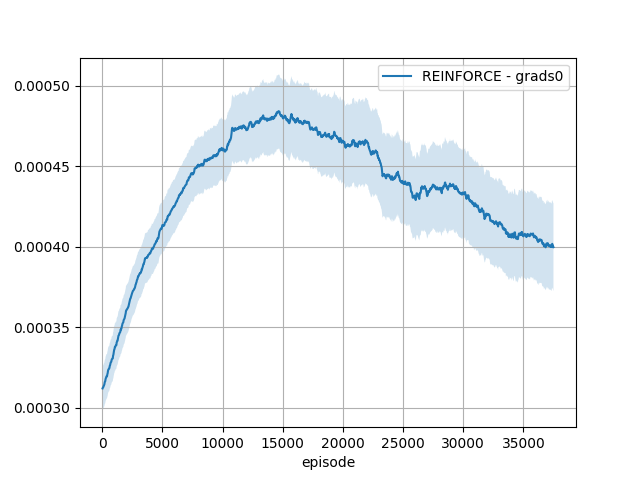
\includegraphics[width=8cm]{images/experiment4/grad0.png}
  \captionof{figure}{Gradient estimate for agent $0$}
  \label{fig:exp1_grad0}
\end{minipage}%
\begin{minipage}{.5\textwidth}
  \centering
  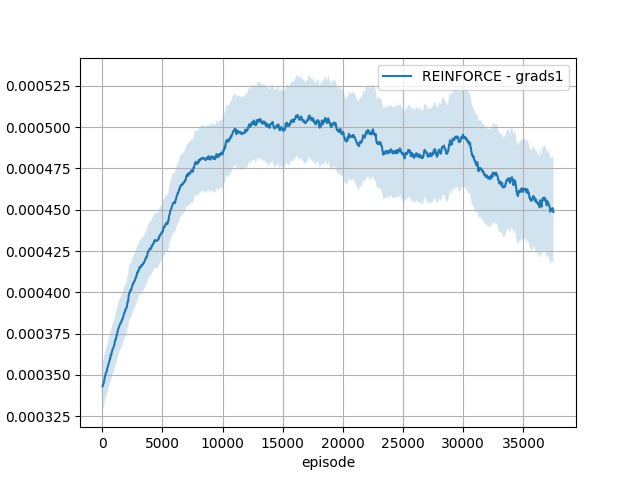
\includegraphics[width=8cm]{images/experiment4/grad1.png}
  \captionof{figure}{Gradient estimate for agent $1$}
  \label{fig:exp1_grad1}
\end{minipage}
\end{figure}

Figure \ref{fig:exp1_length} shows the average duration of an episode. Notice that initially, when the agent's policy network has random weights and the agent effectively behaves as a random agent, the episodes take a long time because none of the agents is taking any directed actions. Once the agent learns from experience, his behavior becomes more directive and the episode duration decreases rapidly. This behavior is encouraged by the fact that the agent receives a small negative reward for every step, incentivizing the agents to reduce the episode length. Figure \ref{fig:exp1_reward} shows the average final reward per episode for the agents\footnote{This is not the cumulative reward, and thus doesn't take into account any negative step rewards}. Initially, the agents lose as often as they win; the reward is negative, partially because agents are penalized for draws (e.g. because they run out of ammo). However, the win rate increases rapidly and finally the agents will win almost all the time. This curve is called the \emph{learning curve} and will be the standard way to evaluate the performance of a MARL algorithm.\\
\begin{figure}
\centering
\begin{minipage}{.5\textwidth}
  \centering
  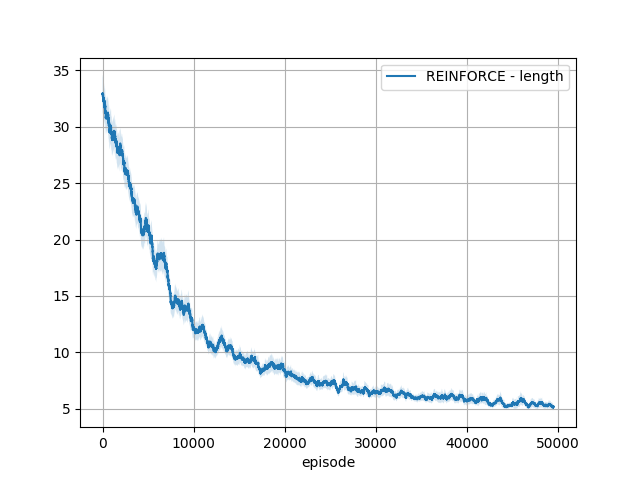
\includegraphics[width=8cm]{images/experiment4/mean_length.png}
  \captionof{figure}{Mean episode length}
  \label{fig:exp1_length}
\end{minipage}%
\begin{minipage}{.5\textwidth}
  \centering
  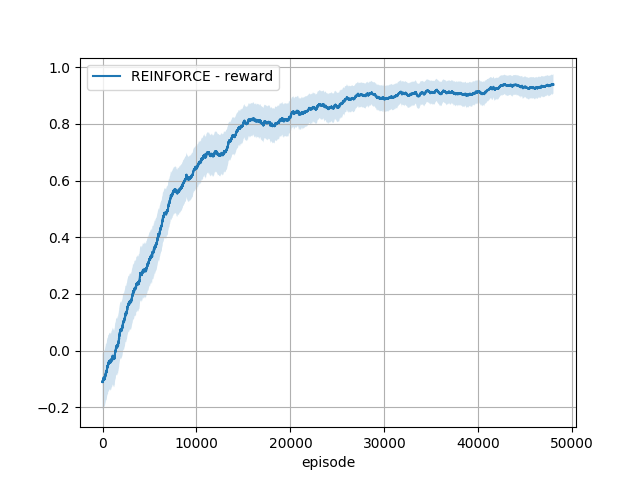
\includegraphics[width=8cm]{images/experiment4/mean_reward.png}
  \captionof{figure}{Mean reward for agents of team 1}
  \label{fig:exp1_reward}
\end{minipage}
\end{figure}

In this simple scenario, the agents have learned to (in this order):
\begin{enumerate}
    \item Aim at the opposing agents (resp. $T0 \rightarrow T2$ and $T1 \rightarrow T3$).
    \item Come closer until the opposing agent is in range.
    \item Fire once the opposing agent is in range.
\end{enumerate}
Figure \ref{fig:simple_tactic01} shows how this is done. A line between agents means one agent is aiming at the other. The actions taken by the four agents are shown in the top left corners.

%\includemovie{8cm}{8cm}{images/tactic01.gif}
% \begin{frame}{}
%   \animategraphics[loop,controls,width=10cm]{10}{images/animation01/screenshot0-}{0}{4}
% \end{frame}

% \begin{frame}
%     \transduration<0-4>{0}
%     \multiinclude[<+->][format=png, graphics={width=10cm}]{images/animation01/screenshot0}
% \end{frame}

\begin{comment}

\begin{figure}
\centering
\begin{minipage}{.5\textwidth}
  \centering
  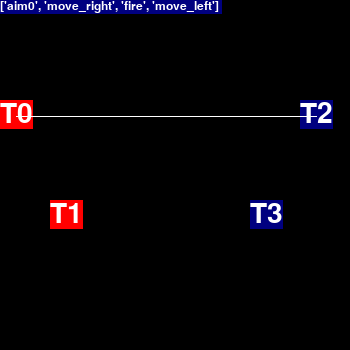
\includegraphics[width=7cm]{images/animation01/screenshot0-1.png}
\end{minipage}%
\begin{minipage}{.5\textwidth}
  \centering
  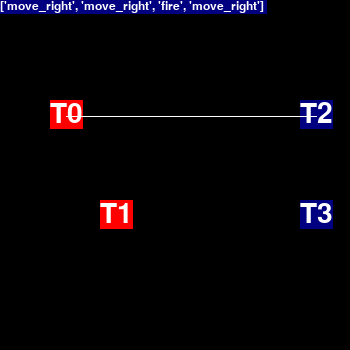
\includegraphics[width=7cm]{images/animation01/screenshot0-2.png}
\end{minipage}
%\end{figure}
%\begin{figure}
\centering
\begin{minipage}{.5\textwidth}
  \centering
  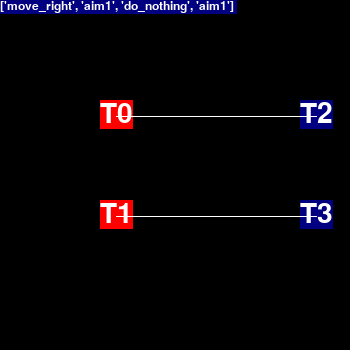
\includegraphics[width=7cm]{images/animation01/screenshot0-3.png}
\end{minipage}%
\begin{minipage}{.5\textwidth}
  \centering
  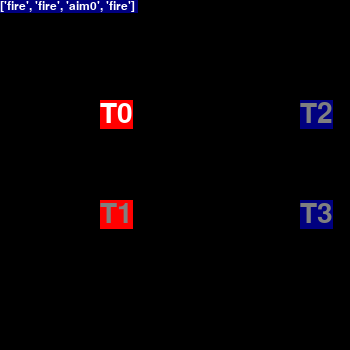
\includegraphics[width=7cm]{images/animation01/screenshot0-4.png}
\end{minipage}
\caption{A simple learned tactic}
\label{fig:simple_tactic01}
\end{figure}

\end{comment}

\begin{figure}[htp]
\centering
\begin{minipage}{.45\textwidth}
  \centering
  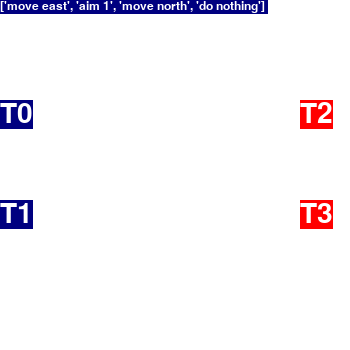
\includegraphics[width=6cm]{images/animation03/screenshot01.png}
  \caption*{Initial positions.}
\end{minipage}%
\begin{minipage}{.1\textwidth}
\centering
  \caption*{ }
\end{minipage}%
\begin{minipage}{.45\textwidth}
  \centering
  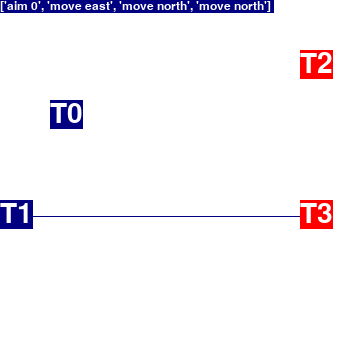
\includegraphics[width=6cm]{images/animation03/screenshot02.png}
  \caption*{ $T0$ moved east, while $T1$ aims at $T3$.}
\end{minipage}
%\end{figure}
%\begin{figure}
\centering
\begin{minipage}{.45\textwidth}
  \centering
  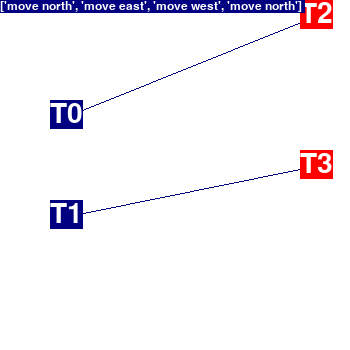
\includegraphics[width=6cm]{images/animation03/screenshot03.png}
  \caption*{The opposite happens: $T0$ aims at $T2$ while $T1$ moved east. Both blue agents are now aiming but are too far away to fire.}
\end{minipage}%
\begin{minipage}{.1\textwidth}
\centering
  \caption*{ }
\end{minipage}%
\begin{minipage}{.45\textwidth}
  \centering
  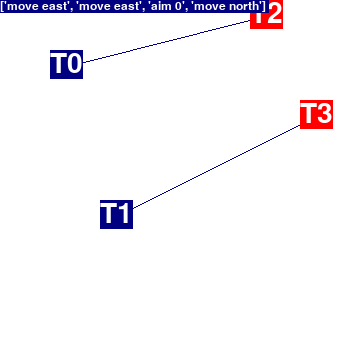
\includegraphics[width=6cm]{images/animation03/screenshot04.png}
    \caption*{Both blue agents keep moving east to get their opponents in fire range.}
\end{minipage}
\begin{minipage}{.5\textwidth}
  \centering
  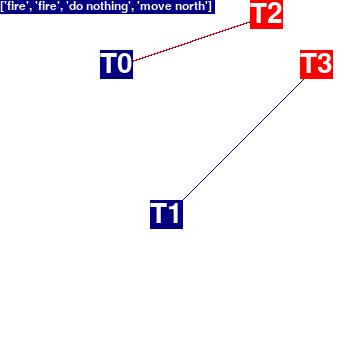
\includegraphics[width=6cm]{images/animation03/screenshot05.png}
    \caption*{Once in range, they both fire.}
\end{minipage}%
\begin{minipage}{.5\textwidth}
  \centering
  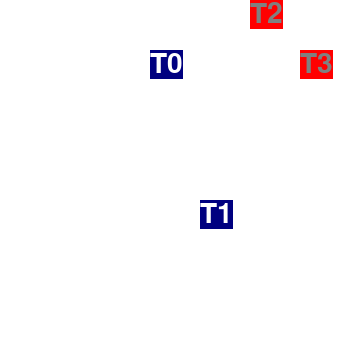
\includegraphics[width=6cm]{images/animation03/screenshot99.png}
  \caption*{Both red agents are dead.}
\end{minipage}
\caption{A simple learned tactic}
\label{fig:simple_tactic01}
\end{figure}

\subsubsection*{Comparison}
The next step consists of comparing the learning curves of the three types of independent learning algorithms: (i) Independent REINFORCE just as above, (ii) Independent Actor-Critic, where REINFORCE is extended with a critic to estimate the state value and (iii) Independent Q-Learning (IQL), where the policy is derived from the Q-value for each action in a state. The resulting learning curves are represented in figure \ref{fig:compare_reward}.

\begin{figure}[htp]
    \centering
    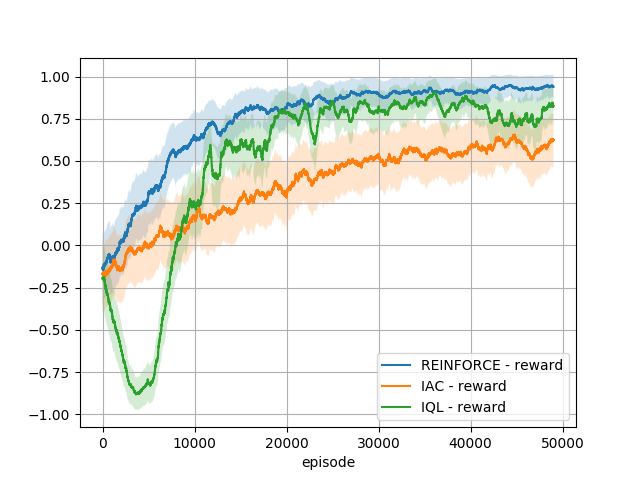
\includegraphics[width=14cm]{images/experiment4/compare_reward.png}
    \caption{Learning rate for REINFORCE, Independent Actor-Critic and IQL for 2v2 games}
    \label{fig:compare_reward}
\end{figure}

The following points are significant:
\begin{itemize}
    \item Out of the 3 algorithms, REINFORCE works best since its learning curve is the steepest and it converges fastest to $1$.
    \item IQL initially goes in the wrong direction (i.e. makes wrong moves) before starting to improve the reward. This is caused by the high initial $\epsilon$ in the $\epsilon$-greedy action selection process which causes the behavior to be random instead of guided by the learned $Q$-values.
    \item To have a fair comparison, Q-learning algorithms will from now on be compared by generating episodes with an $\epsilon = 0$, thus always choosing the action with the highest estimated $Q$-value.
    \item Since IQL derives the policy from the learned $Q$-values, its behavior during learning undergoes significantly higher variation than REINFORCE. This is because gradual changes in $\hat Q(s, a)$ can lead to suddenly preferring one action over another.
    \item The learning curve of Independent Actor-Critic is slower than those for REINFORCE and IQL. This is probably because this algorithm has to learn both a policy and value-estimation function at the same time.
    \item Independent Actor-Critic is highly dependent on the inclusion of an entropy-term to avoid the policy distribution from collapsing to a distribution that puts all probability mass on a single action.
\end{itemize}

Independent REINFORCE definitely works best, and this has been confirmed by numerous experiments. IQL can be an alternative, but as mentioned above, many hyperparameters have to be tuned to achieve good performance. This point will also be addressed when discussing QMix. Independent Actor-Critic performs significantly worse than independent REINFORCE. Why this is the case shall be part of further investigations.\\
In the next section the performance of QMix will be compared against REINFORCE.

\begin{comment}
\textbf{TODO:} Rephrase the paragraph below.\\
The next evolution is to represent the agent as a recurrent neural network as explained in section \ref{sec:deep_pg}. The input of the network are the two major components of the state vector $\bm{s_t}$:
\begin{enumerate}
    \item The game board, namely the actual position of the agent relative to the board and each other, and
    \item Additional information about the agents (are they alive? What is the ammo level?)
\end{enumerate}
The board information is well suited to serve as input of a convolutional layer, since it contains spatial information. The additional information on the other hand will be fed to a fully-connected neural network layer. The result of both these layers is then combined and serves as the input for the a fully-connected layer. The output of this layer is then fed to a GRU. The neural net will have two heads, as explained in section \ref{sec:deep_pg}, and can thus be used in an actor-critic algorithm. An overview of the agent's neural network is shown in figure \ref{fig:agent_net}.
\begin{figure}[htp]
    \centering
    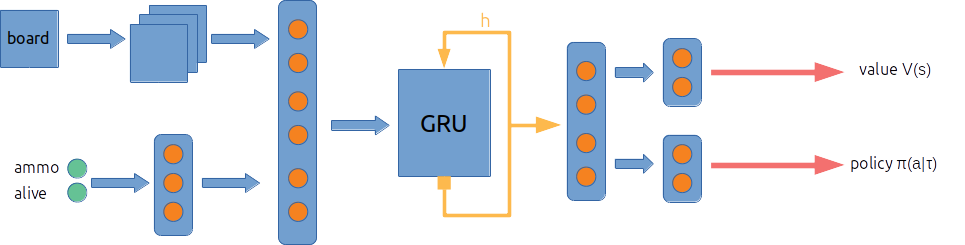
\includegraphics[width=16cm]{images/agent_net.png}
    \caption{Actor-critic agent with recurrent net}
    \label{fig:agent_net}
\end{figure}

While this modification might result in a theoretical improvement, this is not the case in practice. Figure \ref{fig:newplot194_195} shows the learning curve for agents with non-recurrent (blue) and recurrent neural nets (green). While both learn a winning strategy, it is not feasible to say one approach is better than the other. \textbf{TODO}: improve this (correct or explain).

% comparison 194-195
\begin{figure}[htp]
    \centering
    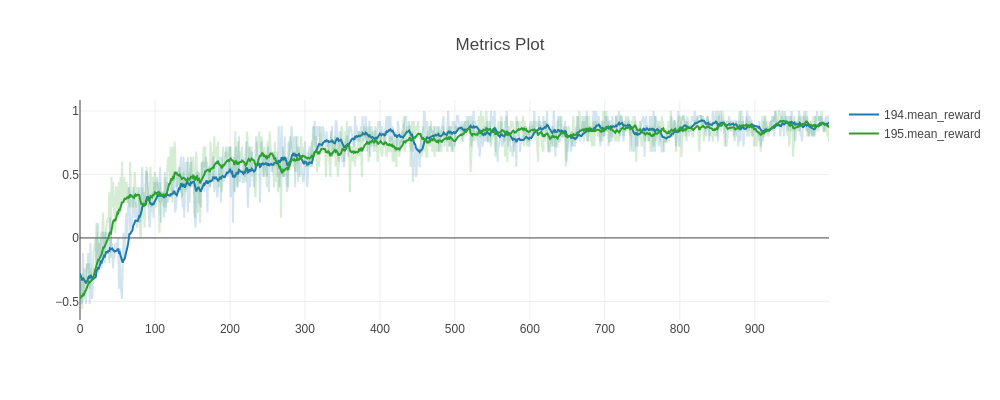
\includegraphics[width=14cm]{images/experiment2/newplot194_195.png}
    \caption{Forward vs. GRU Network}
    \label{fig:newplot194_195}
\end{figure}

%insert comparison PG (run ideapad 582) and IQL (run ideapad 590)
\end{comment}

\subsection{QMix}
\label{sec:init_model_qmix}
As explained in section \ref{sec:intro_qmix}, QMix is an algorithm of the Q-learning family that combines the Q-value estimate of the different agents into a $Q_{tot}$ such that $\frac{\partial Q_{tot}}{\partial Q_i} \geq 0$ for all agents $i$. This guarantees that when each agent chooses his best action $a_i$, the combined action set $[a_1 \ldots a_N]$ will also be the best possible joint action for the team.\\
QMix uses during training the state information $s_t$ to set the weights of the mixing network in figure \ref{fig:qmix_structure}. To do this, the state information was transformed in a tensor of size {\tt n\_agents x 5}, where each agent is represented by 5 items: his position $(x, y)$, whether he is still alive, his ammo level and at whom he is aiming at (if that is the case).\\
Figure \ref{fig:comp_qmix_pg} compares the learning curve of REINFORCE with the one for QMix.
% comparison 396-419
\begin{figure}[htp]
    \centering
    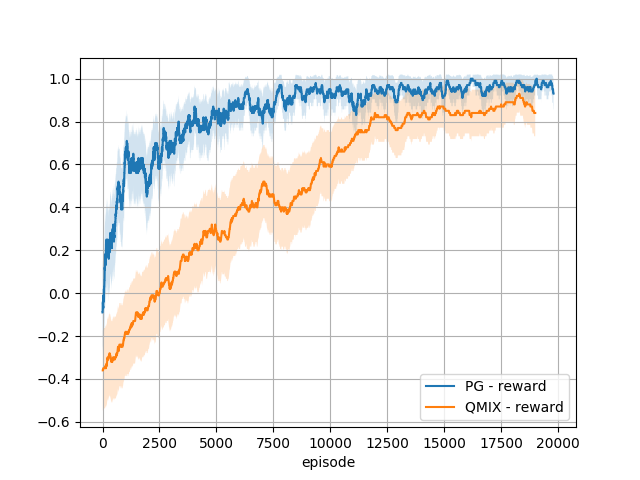
\includegraphics[width=14cm]{images/experiment5/pg_v_qmix_simple.png}
    \caption{QMix vs independent REINFORCE in a simple environment}
    \label{fig:comp_qmix_pg}
\end{figure}
Both algorithms convergence to a situation where the blue team wins the large majority of its games. However, independent REINFORCE clearly works better, both in sample efficiency (since its curve is steeper) and in final reward which on average is much closer to $1$. Indeed, investigation of the resulting strategies didn't show anything better than REINFORCE produced. However, QMix is an algorithm that encourages cooperation between agents and its advantages should become clearer when we look at the extended environment.\\
Experimentation has shown a few remarkable facts:
\begin{enumerate}
    \item The discount factor $\gamma$ is a critical parameter: policy gradient algorithms like REINFORCE require a high $\gamma$ (around $0.99$), while Q-learning based algorithms like IQL and QMix only converge when $\gamma$ is lower ($0.8$ and below). A possible reason might be that PG algorithms base their update on a sequence of steps of a single episode, while Q-learning algorithms take random samples out a buffer of steps coming from multiple episodes. This means that the temporal effect of actions is more pronounced for PG and this can have an impact on the sensitivity on $\gamma$. However, this explanation has not been confirmed. The issue will be part of future research.
    \item Convergence of QMix is much better when the step penalty is increased and the maximum episode length is kept low. REINFORCE in turn has no problem to converge with a lower (or even zero) step penalty.
\end{enumerate}

\section{Extended Model}
\label{sec:init_model_applied}
This section describes the obtained results when the different algorithms are applied to the second model of which the characteristics were sketched in section \ref{sec:extended_model}.\\
A new model also requires that a couple of technical points be addressed:
\begin{itemize}
    \item Environments can host a number of agents that is not predefined. This implies that the action space must be dynamical since the number of {\tt aim}-actions depends on the number of opposing agents. Hence the number of outputs of the policy- or Q-value network changes. This issue was already addressed in chapter \ref{ch:modelling}.
    \item An additional requirement for being allowed to fire is that the opposing agent is visible, i.e. the line-of-sight is not blocked by an obstacle or other agent. This is communicated to the network by adding additional flags to the observation tensor, one flag per opponent that says whether he's visible or not.
    \item The terrain is added to the observation. Since the terrain doesn't change during play, this information is not stored when generating the episodes because that would waste resources. The information is appended to the observation matrix when it is offered to the network.\\
    For a board size $n$, this means an addition of $n^2$ elements to the input of the network, and thus also a severe increase in the number of network weights in the initial layer. This can be alleviated by using a convolutional network to process the board (containing both agents and terrain). This will be part of future research.
\end{itemize}

\subsection{Independent RL}
REINFORCE works reasonably well with the extended model. Figure \ref{fig:pg_extended} shows both win rate and average length for REINFORCE applied to the extended model with a large obstacle in the middle (like in figure \ref{fig:simple_tactic02}) on a 15-by-15 board, which is more than 4 times larger than the simple model. 
\begin{figure}[htp]
\centering
\begin{minipage}{.45\textwidth}
  \centering
  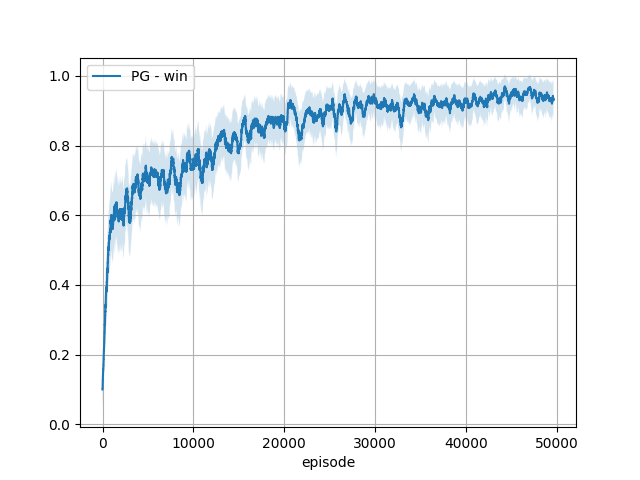
\includegraphics[width=8cm]{images/experiment6/pg_win_15.png}
\end{minipage}%
\begin{minipage}{.05\textwidth}
\centering
  \caption*{ }
\end{minipage}%
\begin{minipage}{.45\textwidth}
  \centering
  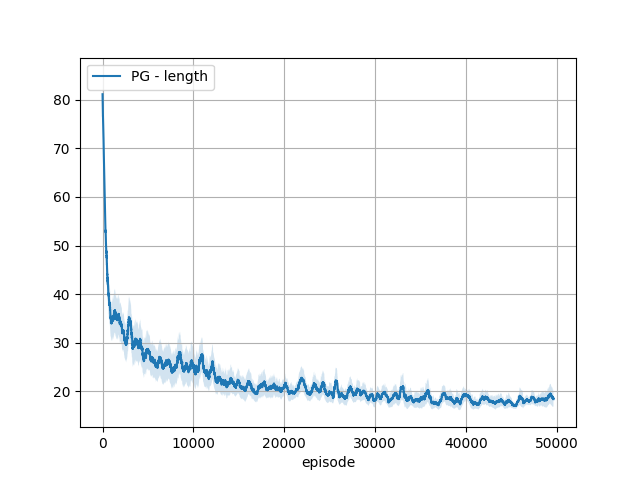
\includegraphics[width=8cm]{images/experiment6/pg_length_15.png}
\end{minipage}
\caption{Win rate and average game length for REINFORCE on extended model 15-by-15 board}
\label{fig:pg_extended}
\end{figure}
It takes about $20000$ episodes to reach a $90\%$ win rate; compare this with figure \ref{fig:comp_qmix_pg} where REINFORCE requires about $6000$ episodes to reach the same level of wins. However, increasing the board size with a factor of $4$ entails an increase of the state-space size by a factor $\approx 4^4 = 256$ (since each of the $4$ players can be placed on $4$ times as many tiles). In this light the increase in required samples seems reasonable.\\
Another test is whether we can learn to win in a situation of 2 blue agents against 3 red ones, putting the blue team at a serious disadvantage. Figure \ref{fig:pg_extended2} shows both the win rate and the episode length for this situation. These curves show that winning in that situation is definitely possible - although still against random agents - but notice that (compare with figure \ref{fig:comp_qmix_pg}) the curve is a lot less steep, especially in the beginning. This would indicate that the algorithm needs a lot of episodes to figure out how to beat $3$ opponents with $2$ agents.

\begin{figure}[htp]
\centering
\begin{minipage}{.45\textwidth}
  \centering
  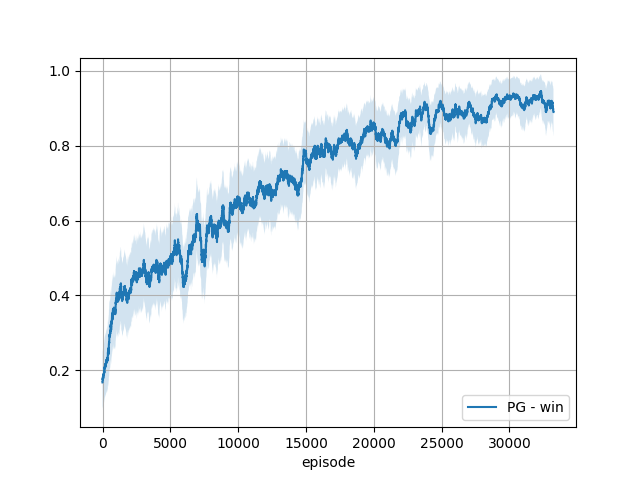
\includegraphics[width=8cm]{images/experiment6/pg_win_2v3.png}
\end{minipage}%
\begin{minipage}{.05\textwidth}
\centering
  \caption*{ }
\end{minipage}%
\begin{minipage}{.45\textwidth}
  \centering
  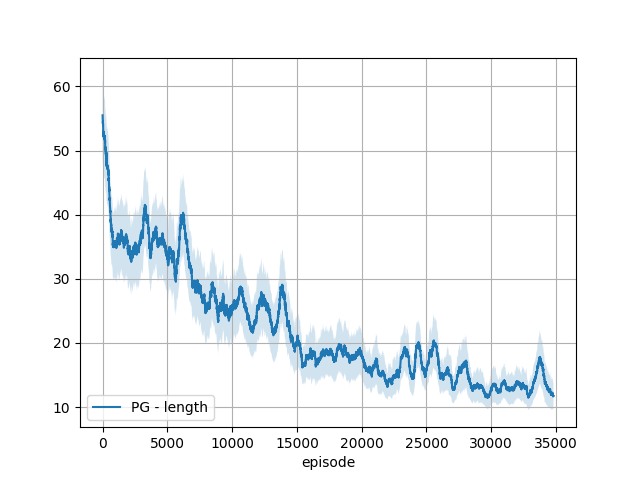
\includegraphics[width=8cm]{images/experiment6/pg_length_2v3.png}
\end{minipage}
\caption{Win rate and average game length for REINFORCE on extended model 2v3 agents}
\label{fig:pg_extended2}
\end{figure}

Figure \ref{fig:simple_tactic02} shows the play-out of a game on a 7-by-7 board with that same large obstacle in the middle. The blue and red lines between agents represent the aiming action of resp. blue and red agents. The action that the agents choose to take based on their current observation are shown in the top left of each figure. The captions below the figures explain how the agents behave.

\begin{figure}
\centering
\begin{minipage}{.45\textwidth}
  \centering
  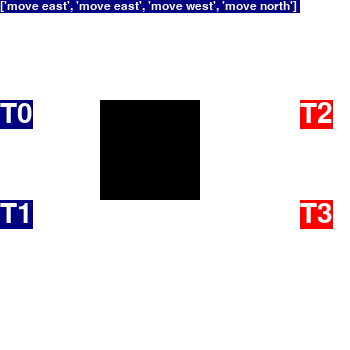
\includegraphics[width=6cm]{images/iteration/screenshot01.png}
  \caption*{Initial positions with large obstacle in the middle of the board}
\end{minipage}%
\begin{minipage}{.1\textwidth}
\centering
  \caption*{ }
\end{minipage}%
\begin{minipage}{.45\textwidth}
  \centering
  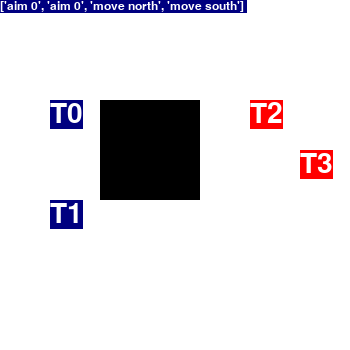
\includegraphics[width=6cm]{images/iteration/screenshot02.png}
  \caption*{Both blue agents take action to aim at $T2$}
\end{minipage}
%\end{figure}
%\begin{figure}
\centering
\begin{minipage}{.45\textwidth}
  \centering
  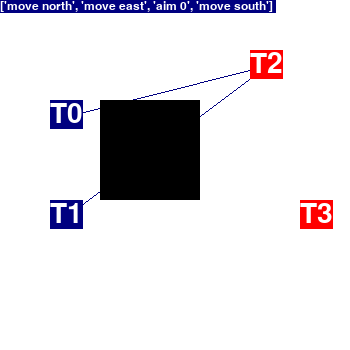
\includegraphics[width=6cm]{images/iteration/screenshot03.png}
  \caption*{Both blue agents are aiming at $T2$ but are not allowed to fire; agent $T0$ moves north to clear line-of-sight}
\end{minipage}%
\begin{minipage}{.1\textwidth}
\centering
  \caption*{ }
\end{minipage}%
\begin{minipage}{.45\textwidth}
  \centering
  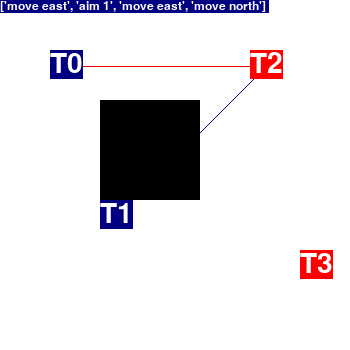
\includegraphics[width=6cm]{images/iteration/screenshot04.png}
    \caption*{$T0$ moves closer to $T2$ to get in fire range; agent $T1$ switches aim to agent $T3$}
\end{minipage}
\begin{minipage}{.5\textwidth}
  \centering
  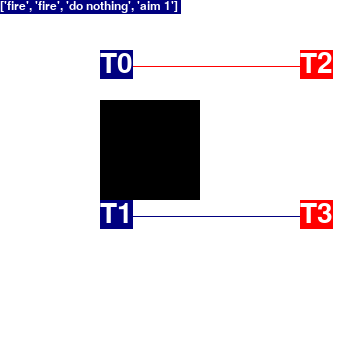
\includegraphics[width=6cm]{images/iteration/screenshot05.png}
    \caption*{Both blue agents fire at opposing agents at the same time, killing both}
\end{minipage}%
\begin{minipage}{.5\textwidth}
  \centering
  %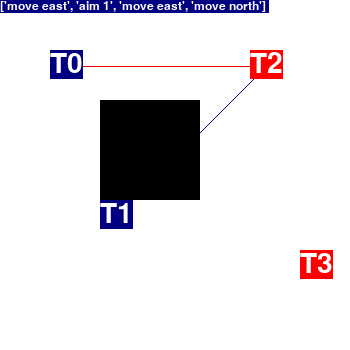
\includegraphics[width=7cm]{images/iteration/screenshot04.png}
\end{minipage}
\caption{A game with an obstacle}
\label{fig:simple_tactic02}
\end{figure}

\subsection{QMix}
QMix works reasonably well on the extended model, as long as the board size is small. Once the board size becomes larger than $11$-by-$11$, it becomes very hard to get QMix to converge. This is unfortunate, since intuitively, cooperation between agents becomes more important when the board size is large.\\
For smaller board sizes, QMix gives quite good results, as can been seen in figure \ref{fig:comp_qmix_pg2} where the learning curve for REINFORCE and QMix is compared on a 9-by-9 board with obstacles in the terrain (a figure which is the counterpart of figure \ref{fig:comp_qmix_pg}).

\begin{figure}[htp]
    \centering
    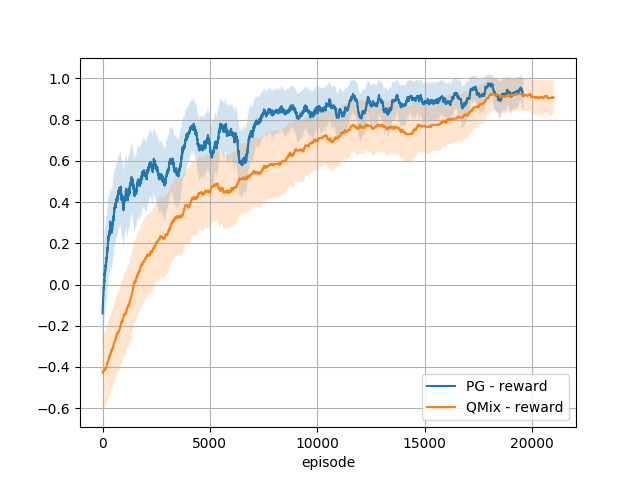
\includegraphics[width=14cm]{images/experiment6/qmix_vs_pg_win_9.png}
    \caption{QMix vs independent REINFORCE on a 9-by-9 board}
    \label{fig:comp_qmix_pg2}
\end{figure}

Notice that although being slower, QMix still reaches the $90\%$ win rate in about $17000$ episodes, which is reasonably compared to REINFORCE. Nevertheless, the conclusion remains that QMix lacks scalability, an issue that has not been resolved.

\section{Model Transfer}
\label{sec:model_transfer}
Obtaining a model that performs well against an opponent that deploys a random strategy is one thing. More interesting things can happen when we train against more advanced agents. To do so, the neural network and its inputs on which an agent relies to choose his action has been constructed in such a way that:
\begin{itemize}
    \item agents of the same team share the same network (weight sharing), and
    \item agents of the opposing team can reuse that trained network to obtain the same performance as the other team
\end{itemize}
In this way, we can swap the trained network from the blue team to the red one to get an opponent that doesn't behave randomly but uses a (slightly) smarter strategy. By doing this in an iterative fashion we continuously improve our strategy. More concretely:
\begin{enumerate}
    \item Start training the blue team against a random opponent;
    \item After a certain number of steps or once the blue team consistently beats the red one, transfer the network from the blue team to the red one;
    \item Continue improving the blue team against the better opponent. Either start from a clean network or keep the already trained network. The former option might be useful to avoid getting stuck in a local minimum where the learned strategy is too brittle and only works in a limited number of cases. The latter option is obviously more sample efficient.
    \item Go back to step 2.
\end{enumerate}
Going forward, all figures were produced on a 7-by-7 board with teams of 2 agents and a terrain containing several obstacles.\\
Figure \ref{fig:iteration} shows the win rate for both blue and red teams where after each 5000 episodes the network was transferred to the red team and the agents from the blue team restarted training as random agents. The performance loss for the blue team - and the corresponding performance gain for the red team - is clearly visible every 5000-episode cycle. During some cycles (e.g. from episode $10000$ to $15000$) it is hard to overcome the opponent while during other cycles the blue team easily overcomes the red one (e.g. from episode $15000$ to $20000$).\\
\begin{figure}[htp]
    \centering
    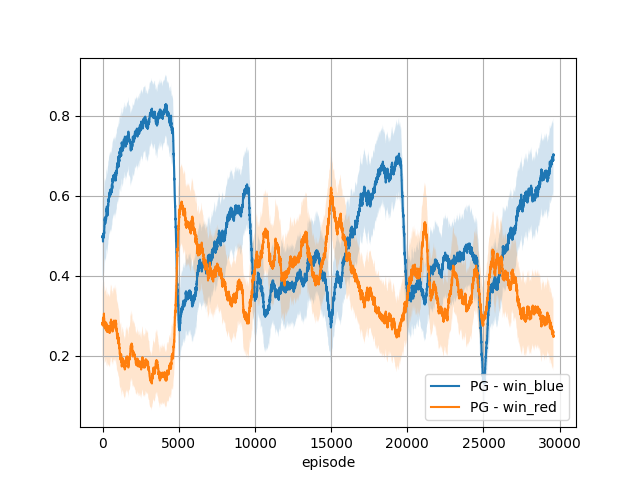
\includegraphics[width=14cm]{images/iteration/iterative.png}
    \caption{Sequence of model transfers from team blue to team red}
    \label{fig:iteration}
\end{figure}
Figure \ref{fig:iterative_qmix} is a rather striking example of the transfer of a QMix model from blue to red whilst keeping the model for the blue team. A word of caution: this simulation ran for 60000 episodes, but a performance evaluation was only done every 10 episodes, thus the $x$-axis reports only 6000 episodes (actually a bit less because of the moving-window averaging with window size $=400$).
\begin{figure}[htp]
    \centering
    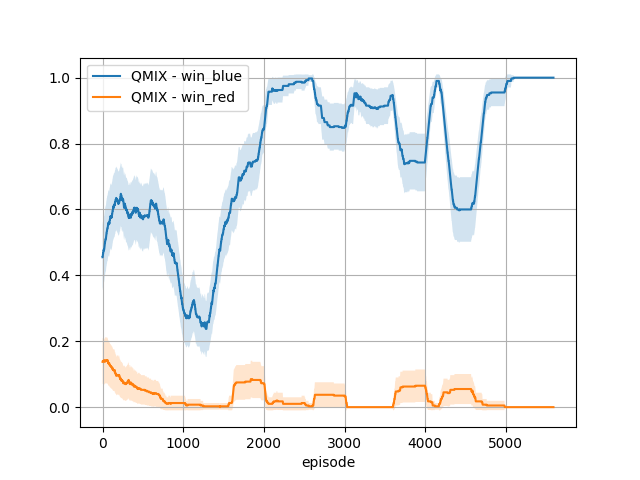
\includegraphics[width=14cm]{images/iteration/iterative_qmix.png}
    \caption{Sequence of model transfers for QMix - no network reset}
    \label{fig:iterative_qmix}
\end{figure}
It is clear when the red team receives a new network since the performance briefly flares up. However, the blue performance remains relatively high during the entire sequence, a part from the occasional drop when the blue network is shared and the blue agents essentially have to compete against themselves.




% TODO: explain model transfering from friend to foe
% TODO (maybe) discuss transferability over different terrains
% python3 qmix.py with gamma=0.9 qmix_ns=True max_episode_length=20 step_penalty=0.1 lr=0.001 % n_steps=50000 > /dev/null &
